\section{Model matematyczny}
\indent

W~poniższym rozdziale przedstawiona została konstrukcja modelu matematycznego
układu chłodzenia cieczą procesora komputera oraz wyznaczanie odpowiednich
parametrów tego modelu.

Na podstawie informacji znalezionych na stronie \cite{EKWBsite} oraz na forach
zajmujących się tematyką chłodzenia wodnego komputera, możliwe było
zaprojektowanie prostej pętli, w~skład której wchodził blok wodny, którego
zadanie polegało na odbieraniu ciepła z~powierzchni procesora oraz radiator
(chłodnica) oddający ciepło do otoczenia. Dodatkowym niezbędnym elementem była
pompa wymuszająca obieg wody w~układzie oraz wentylatory umieszczone na
radiatorze wspomagające przepływ powietrza.

Równania różniczkowe opisujące powyższe elementy układu chłodzenia przedstawione
są w~kolejnych podrozdziałach. Do ich konstrukcji (w~przypadku opisu przepływu
ciepła) zastosowane zostało prawo Fouriera przy pewnych założeniach:
\begin{itemize}
    \item materiały, z~których wykonany jest blok wodny oraz chłodnica są
    jednorodne,
    \item w~związku z~powyższym, przepływ ciepła przez te materiały również jest
    jednorodny,
    \item matematyczny opis wymiany ciepła jest uproszczony.
\end{itemize}

\subsection{Równania pompy i~wentylatorów}
\indent

Pompa wody oraz wentylatory w~układach chłodzenia cieczą są zwykle zasilane
z~jednego z~napięć dostarczanych przez zasilacz komputera --~$5$ lub $12$~[$V$],
w~zależności od producenta. Rodzaj wykorzystanych silników oraz sposób
sterowania nimi nie był jednak tematem tej pracy, przez co przyjęte zostały
pewne uproszczenia odnośnie sterowania --~pomijany jest dokładny sposób
zasilania oraz opis matematyczny. Założenie polegało na przyjęciu, iż zarówno
zachowanie silnika pompy jak i~wentylatorów można z~pewnym przybliżeniem
przedstawić w~postaci równania różniczkowego pierwszego rzędu --~jako inercję
pierwszego rzędu. Wartości sterowań określały natomiast współczynnik
wypełnienia dla sygnałów PWM wykorzystywanych w~układach zasilania silników.

Wentylatory umieszczone na chłodnicy wykorzystywały wspólny sygnał zasilający,
przez co można je było traktować w~uproszczeniu jako jeden większy wentylator
o~odpowiednio dobranych parametrach. W~związku z~tym, do układu doprowadzane
były dwa sygnały sterujące:
\begin{itemize}
    \item $u_1$ --~sygnał sterujący pompą wody,
    \item $u_2$ --~sygnał sterujący wentylatorami,
\end{itemize}
gdzie $u_i \in \left[ 0; 1 \right]$, $i = 1, 2$.

Modele przyjęte dla pompy oraz wentylatorów były inercjami pierwszego rzędu,
a~zatem --~dobierając odpowiednie wzmocnienia --~równania różniczkowe opisujące
te obiekty przedstawiały się następująco:
\begin{equation}
    \dot{x_1} = k_w \cdot \left( u_1 - x_1 \right)
    \label{equ:x1}
\end{equation}
\begin{equation}
    \dot{x_2} = k_a \cdot \left( u_2 - x_2 \right)
    \label{equ:x2}
\end{equation}
gdzie:
\begin{itemize}
    \item $x_1$ --~prędkość obrotowa pompy wody,
    \item $x_2$ --~prędkość obrotowa wentylatorów,
    \item $k_w = 2$ --~współczynnik wzmocnienia dla pompy,
    \item $k_a = 1.25$ --~współczynnik wzmocnienia dla wentylatorów.
\end{itemize}

Wartości prędkości obrotowych, zarówno pompy jak i~wentylatorów, zawierały się
w~przedziale $x_i \in \left[ 0; 1 \right]$, $i = 1, 2$, co wynika wprost
z~równań \eqref{equ:x1} oraz \eqref{equ:x2}. Odpowiednie współczynniki
skalujące wpływające na przepływ wody lub powietrza zostały pobrane ze
specyfikacji przykładowej pompy \cite{EKWBpump} oraz wentylatora \cite{EKWBfan}
i~umieszczone w~równaniach, które wykorzystują te przepływy --~wartości $F_i
\text{,} \quad i \in \left\{ w, a \right\}$ w~równaniu \eqref{equ:x4} oraz
\eqref{equ:x5}. Natomiast współczynniki wzmocnienia dla pompy i~wentylatorów
zostały dobrane jedynie w~taki sposób, aby zróżnicować zachowanie tych elementów
układu.

\subsection{Równanie temperatury struktury krzemowej procesora}
\indent

W~celu wyznacznia równania opisującego przepływ ciepła przez blok wodny
wykorzystane zostało pojęcie rezystancji termicznej \cite{ThermalResistance}.
Opisana jest ona równaniem:
\begin{equation}
    R_{th} = \frac{\Delta T}{Q}
    \label{equ:thermalresistance}
\end{equation}
gdzie:
\begin{itemize}
    \item $R_{th}$ --~rezystancja termiczna materiału,
    \item $\Delta T$ --~różnica temperatur między powierzchniami materiału,
    \item $Q$ --~ilość energii cieplnej przepływającej przez materiał
    w~jednostce czasu (moc cieplna).
\end{itemize}

Rezystancja termiczna jest zwykle bardzo trudna do wyznaczenia, gdyż zależy od
wielu czynników. W~przypadku prostych elementów lub układów elektronicznych,
takich jak diody wysokoprądowe, tranzystory, wzmacniacze scalone i~inne, jest
ona podawana w~notach katalogowych tych elementów. Niestety znalezienie tego
parametru dla obudowy procesora komputerowego i~bloku wodnego nie należy już do
tak prostych, gdyż producenci nie umieszczają takich informacji w~dostępnych
publicznie broszurach.

W~takiej sytuacji, rezystancja bloku wodnego oraz obudowy procesora (jako
całości) została wyznaczona korzystając z~tego, że takie układy w~rzeczywistości
istnieją i~funkcjonują prawidłowo. Typowa maksymalna wartość mocy cieplnej
wydzielanej przez procesor dla najbardziej wydajnych konstrukcji wynosi
$Q_{max} = 140$~[$W$] --~jako przykład został wykorzystany procesor
\textit{Intel i7-5960X} \cite{Inteli7}. Maksymalna dopuszczalna temperatura
złącza krzemowego wynosi zwykle $T_{CPU_{max}} = 100$~[$^\circ C$]. Maksymalna
temperatura wody w~układzie chłodzenia jest uzależniona od konstrukcji pompy
i~jej odporności. Na przykładzie pompy \textit{EK-D5 PWM G2 Motor}, której
specyfikacja znajduje się na stronie \cite{EKWBpump}, wartość tej temperatury
wynosi $T_{w_{max}} = 60$~[$^\circ C$]. Przy założeniu stałej temperatury
struktury krzemowej procesora, cała energia cieplna jest transportowana przez
obudowę i~blok do wody, tak więc rezystancja termiczna wynosi:
\begin{equation}
    R_{th} = \frac{T_{CPU_{max}} - T_{w_{max}}}{Q_{max}} = \frac{100 - 60}{140}
    \left[ \frac{^\circ C}{W} \right] \approx 0.3 \left[ \frac{^\circ C}{W}
    \right]
    \label{equ:wbresistance}
\end{equation}

W~przypadku braku równowagi termodynamicznej, czyli gdy ilość energii
wydzielanej w~strukturze procesora jest różna od odbieranej przez wodę,
następuje zmiana temperatury struktury krzemowej. Opisywana jest ona następującą
zależnością:
\begin{equation}
    K_1 \cdot \Delta T_{CPU} = Q_{IN} - \frac{T_{CPU} - T_c}{R_{th}}
    \label{equ:dtcpu}
\end{equation}
gdzie:
\begin{itemize}
    \item $K_1$ --~współczynnik zmian temperatury struktury krzemowej procesora,
    \item $\Delta T_{CPU}$ --~przyrost temperatury struktury krzemowej
    w~jednostce czasu,
    \item $T_{CPU}$ --~aktualna temperatura struktury krzemowej procesora,
    \item $T_c$ --~aktualna temperatura wody wypływającej z~bloku wodnego (wody
    ciepłej).
\end{itemize}

Współczynnik zmian temperatury struktury krzemowej jest zależny od dwóch
czynników --~masy tej struktury oraz jej ciepła właściwego. Wartości te wynoszą
odpowiednio:
\begin{itemize}
    \item $m_{CPU} = 0.01$~[$kg$],
    \item $c_{CPU} = 710$~[$\frac{J}{kg \cdot K}$]
\end{itemize}
Masa struktury została przyjęta na podstawie średnich wartości wag procesorów,
które zostały znalezione w~różnych źródłach internetowych (przy pominięciu masy
laminatu i~obudowy). Natomiast ciepło właściwe struktury jest równe ciepłu
właściwemu krzemu. Zmieniając oznaczenia zmiennych uzyskano następującą
zależność, która jest równaniem różniczkowym opisującym zmiany temperatury
struktury krzemowej procesora:
\begin{equation}
    \dot{x_3} = \frac{Q_{IN}}{m_{CPU} \cdot c_{CPU}} - \frac{x_3 - x_4}{m_{CPU}
    \cdot c_{CPU} \cdot R_{th}}
    \label{equ:x3}
\end{equation}
gdzie:
\begin{itemize}
    \item $x_3$ --~temperatura struktury krzemowej,
    \item $x_4$ --~temperatura wody wypływającej z~bloku wodnego (wody ciepłej).
\end{itemize}

\newpage

\subsection{Równanie wody ciepłej}
\indent

Woda ciepła w~układzie chłodzenia to woda wypływająca z~bloku wodnego
i~płynąca z~niego do chłodnicy. W~stanie ustalonym ilość energii cieplnej
przekazywanej w~jednostce czasu przez blok wodny ze struktury procesorowej jest
równa energii odbieranej przez wodę w~tym bloku:
\begin{equation}
    \frac{T_{CPU} - T_c}{R_{th}} = K_2 \cdot \left( T_c - T_z \right)
    \label{equ:hotwater}
\end{equation}
gdzie:
\begin{itemize}
    \item $K_2$ --~współczynnik odbierania ciepła przez wodę w~bloku wodnym,
    \item $T_z$ --~temperatura wody wpływającej do bloku wodnego (wody zimnej).
\end{itemize}

Wartość współczynnika $K_2$ zależna jest od ciepła właściwego wody oraz masy
wody przepływającej przez blok wodny w~jednostce czasu:
\begin{equation}
    K_2 = m_{wb} \cdot c_w
    \label{equ:k2}
\end{equation}
Ilość wody przepływającej przez blok wodny jest zależna od aktualnej prędkości
obrotowej pompy wody --~na podstawie równania \eqref{equ:x1} --~oraz jej
wydajności:
\begin{equation}
    m_{wb} = x_1 \cdot m_{wb_{max}}
    \label{equ:mwb}
\end{equation}
W~specyfikacji przykładowej pompy \cite{EKWBpump} producent informuje, iż jej
wydajność wynosi $F_w = 1500$~[$\frac{l}{h}$], czyli $F_w =
\frac{1.5}{3600}$~[$\frac{m^3}{s}$], natomiast gęstość wody jest równa $\rho_w
= 1000$~[$\frac{kg}{m^3}$], co prowadzi do zależności:
\begin{equation}
    m_{wb_{max}} = F_w \cdot \rho_w
    \label{equ:mwbmax}
\end{equation}

Podstawiając powyższe do równania \eqref{equ:hotwater} otrzymano następującą
zależność, która obowiązuje w~stanie ustalonym --~przy ilość energii oddawanej
w~jednostce czasu przez procesor równej ilości odbieranej przez wodę:
\begin{equation}
    \frac{T_{CPU} - T_c}{R_{th}} = x_1 \cdot F_w \cdot \rho_w \cdot c_w \cdot
    \left( T_c - T_z \right)
    \label{equ:hotwaterfull}
\end{equation}
W~sytuacji, gdy układ ten nie znajduje się w~równowadze termodynamicznej
następuje zmiana temperatury wody ciepłej, która opisana jest poniższym
równaniem:
\begin{equation}
    K_3 \cdot \Delta T_c = \frac{T_{CPU} - T_c}{R_{th}} - x_1 \cdot F_w \cdot
    \rho_w \cdot c_w \cdot \left( T_c - T_z \right)
    \label{equ:dtc}
\end{equation}
gdzie:
\begin{itemize}
    \item $K_3$ --~współczynnik zmian temperatury wody ciepłej,
    \item $\Delta T_c$ --~przyrost temperatury wody ciepłej w~jednostce czasu.
\end{itemize}

Wartość współczynnika $K_3$ jest zależna od masy wody w~bloku wodnym oraz
ciepła właściwego wody:
\begin{itemize}
    \item $m_b = 0.15$~[$kg$],
    \item $c_b = 4190$~[$\frac{J}{kg \cdot K}$].
\end{itemize}
Masa wody została przyjęta na podstawie uśrednionych wartości znalezionych na
stronach producentów i~forach. Przyjmując odpowiednie oznaczenia otrzymano
następującą zależność, która jest równaniem różniczkowym opisującym zmiany
temperatury wody wypływającej z~bloku wodnego --~wody ciepłej:
\begin{equation}
    \dot{x_4} = \frac{x_3 - x_4}{m_b \cdot c_b \cdot R_{th}} - x_1 \cdot F_w
    \cdot \rho_w \cdot c_w \frac{x_4 - x_5}{m_b \cdot c_b}
    \label{equ:x4}
\end{equation}

\subsection{Równanie wody zimnej}
\indent

Woda zimna w~układzie chłodzenia to woda, która wypływa z~chłodnicy i~płynie
z~niej do bloku wodnego. W~stanie ustalonym ilość energii cieplnej
transportowana przez wodę ciepłą w~jednostce czasu jest równa ilości energii
rozpraszanej do otoczenia przez radiator:
\begin{equation}
    x_1 \cdot F_w \cdot \rho_w \cdot c_w \cdot \left( T_c - T_z \right) = K_4
    \cdot \left( T_z - T_o \right)
    \label{equ:coldwater}
\end{equation}
gdzie:
\begin{itemize}
    \item $K_4$ --~wpółczynnik odbierania ciepła przez radiator,
    \item $T_o$ --~temperatura otoczenia.
\end{itemize}

W~przypadku radiatora wartość współczynnika $K_4$ jest sumą dwóch wartości:
\begin{itemize}
    \item $K_{41}$ --~współczynnik swobodnego przepływu powietrza,
    \item $K_{42}$ --~współczynnik wymuszonego przepływu powietrza.
\end{itemize}

Wartość współczynnika $K_{41}$ wynika z~naturalnego zjawiska jakim jest
konwekcja. Zgodnie z~informacjami zawartymi na stronie \cite{CHT} wynosi on:
\begin{equation}
    K_{41} = h_a \cdot A_r
    \label{equ:k41}
\end{equation}
gdzie:
\begin{itemize}
    \item $h_a$ --~współczynnik przenikania ciepła,
    \item $A_r$ --~efektywna powierzchnia radiatora.
\end{itemize}
Wartość współczynnika $h_a$ dla swobodnego przepływu ciepła, według informacji
zawartych na stronie \cite{CHT}, powinna wynosić w~najmniej korzystnym przypadku
$h_a = 0.5$~[$\frac{W}{m^2 \cdot K}$]. Na potrzeby tego układu została ona
jednak jeszcze bardziej zmniejszona z~powodu budowy chłodnicy oraz umieszczenia
na niej wentylatorów, a~co za tym idzie, utrudnień w~swobodnym przepływie
powietrza. Ostatecznie przyjęta została wartość $h_a = 0.1$~[$\frac{W}{m^2
\cdot K}$].

W~przypadku tworzonego układu wybrana została chłodnica o~parametrach
identycznych jak fizycznie dostępny produkt \cite{EKWBradiator}:
\begin{itemize}
    \item $l = 0.52$~[$m$] --~długość,
    \item $w = 0.13$~[$m$] --~szerokość,
    \item $h = 0.038$~[$m$] --~wysokość,
    \item $FPI = 19$~[$\frac{1}{in}$] --~liczba finów (żeberek) na cal.
\end{itemize}
Powierzchnia efektywna chłodnicy zależy nie tylko od jej fizycznych wymiarów,
ale w~dużej mierze od parametru $FPI$. Wpływ wartości tego parametru na budowę
chłodnicy przedstawiony jest na rysunku~\ref{fig:fpicomp}, gdzie widoczny jest
fragment chłodnicy --~widok ,,od przodu''.
\begin{figure}[ht]
    \centering
    \begin{subfigure}{.45\textwidth}
        \centering
        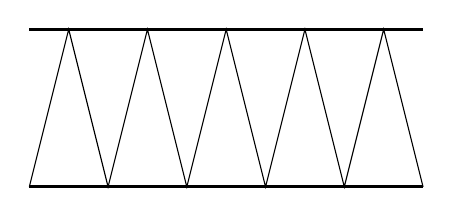
\begin{tikzpicture}
            \draw[very thick] (0, 1) -- (5, 1);
            \draw[very thick] (0, -1) -- (5, -1);
            \draw (0, -1) -- ++(.5, 2) -- ++(.5, -2) -- ++(.5, 2) -- ++(.5, -2)
            -- ++(.5, 2) -- ++(.5, -2) -- ++(.5, 2) -- ++(.5, -2) -- ++(.5, 2)
            -- ++(.5, -2);
        \end{tikzpicture}
        \caption{$FPI = FPI_a$}
    \end{subfigure}
    \begin{subfigure}{.45\textwidth}
        \centering
        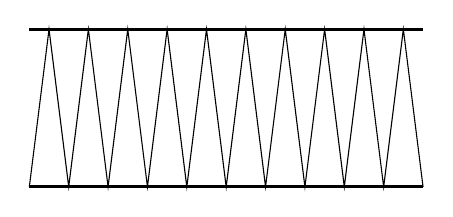
\begin{tikzpicture}
            \draw[very thick] (0, 1) -- (5, 1);
            \draw[very thick] (0, -1) -- (5, -1);
            \draw (0, -1) -- ++(.25, 2) -- ++(.25, -2) -- ++(.25, 2) -- ++(.25,
            -2) -- ++(.25, 2) -- ++(.25, -2) -- ++(.25, 2) -- ++(.25, -2) --
            ++(.25, 2) -- ++(.25, -2) -- ++(.25, 2) -- ++(.25, -2) -- ++(.25, 2)
            -- ++(.25, -2) -- ++(.25, 2) -- ++(.25, -2) -- ++(.25, 2) -- ++(.25,
            -2) -- ++(.25, 2) -- ++(.25, -2);
        \end{tikzpicture}
        \caption{$FPI = FPI_b$}
    \end{subfigure}
    \caption{Porównanie wpływu współczynnika $FPI$ na budowę i~efektywną
    powierzchnię chłodnicy --~$FPI_a < FPI_b$}
    \label{fig:fpicomp}
\end{figure}

Wiedząc w~jaki sposób współczynnik $FPI$ wpływa na efektywną powierzchnię
chłodnicy, możliwe było wyznaczenie jej wartości:
\begin{equation}
    A_r = 2 \cdot \left\lfloor l \cdot \frac{FPI}{0.025} \right\rfloor \cdot w
    \cdot h
    \label{equ:radA}
\end{equation}
Mnożenie przez $2$ w~powyższym wzorze wynika z~tego, że finy mają dwie
powierzchnie, dzielenie przez $0.025$ spowodowane jest koniecznością
przeliczenia wartości współczynnika $FPI$ na jednostki metryczne, natomiast
wyznaczanie podłogi było podyktowane koniecznością otrzymania całkowitej liczby
żeberek w~chłodnicy.

Wartość współczynnika $K_{42}$ wynika z~wymuszonego przepływu powietrza
spowodowanego działaniem wentylatorów i~jej wyznaczanie jest analogiczne jak
w~przypadku współczynnika $K_2$ w~równaniu \eqref{equ:k2}:
\begin{equation}
    K_{42} = m_{ar} \cdot c_a
    \label{equ:k42}
\end{equation}
Ilość powietrza przepływającego przez radiator jest zależna od aktualnej
prędkości obrotowej wentylatorów --~na podstawie równania \eqref{equ:x2} --~oraz
ich wydajności:
\begin{equation}
    m_{ar} = x_2 \cdot m_{ar_{max}}
    \label{equ:mar}
\end{equation}
W~specyfikacji przykładowego wentylatora \cite{EKWBfan} producent informuje, że
jego wydajność wynosi $F_a = 181$~[$\frac{m^3}{h}$], czyli $F_a =
\frac{181}{3600}$~[$\frac{m^3}{s}$], natomiast gęstość powietrza równa jest
$\rho_a = 1.2$~[$\frac{kg}{m^3}$]. Wiedząc, że do wybranej chłodnicy można
przymocować cztery wentylatory, ostatecznie wydajność została ustalona na
wartość $F_a = \frac{4 \cdot 181}{3600}$~[$\frac{m^3}{h}$], co prowadzi do
zależności:
\begin{equation}
    m_{ar_{max}} = F_a \cdot \rho_a
    \label{equ:marmax}
\end{equation}

Podstawiając powyższe do równiania \eqref{equ:coldwater} otrzymano następującą
zależność, która obowiązuje w~stanie ustalonym --~przy ilości energii
transportowanej przez wodę ciepłą w~jednostce czasu równą ilości energii
oddawanej przez radiator do otoczenia:
\begin{equation}
    x_1 \cdot F_w \cdot \rho_w \cdot c_w \cdot \left( T_c - T_z \right) = \left(
    h_a \cdot A_r + x_2 \cdot F_a \cdot \rho_a \cdot c_a \right) \cdot \left(
    T_z - T_o \right)
    \label{equ:coldwaterfull}
\end{equation}
W~sytuacji, gdy układ ten nie znajduje się w~równowadze termodynamicznej
następuje zmiana temperatury wody zimnej, która opisana jest poniższym
równaniem:
\begin{equation}
    K_5 \cdot \Delta T_z = x_1 \cdot F_w \cdot \rho_w \cdot c_w \cdot \left( T_c
    - T_z \right) - \left( h_a \cdot A_r + x_2 \cdot F_a \cdot \rho_a \cdot c_a
    \right) \cdot \left( T_z - T_o \right)
    \label{equ:dtz}
\end{equation}
gdzie:
\begin{itemize}
    \item $K_5$ --~współczynnik zmian temperatury wody zimnej,
    \item $\Delta T_z$ --~przyrost temperatury wody zimnej w~jednostce czasu.
\end{itemize}

Wartość współczynnika $K_5$ jest zależna od masy wody w~chłodnicy oraz jej
ciepła właściwego:
\begin{itemize}
    \item $m_r = 0.235$~[$kg$],
    \item $c_r = 4190$~[$\frac{J}{kg \cdot K}$].
\end{itemize}
Masa wody została przyjęta na podstawie pojemności chłodnicy zawartej
w~specyfikacji umieszczonej na stronie \cite{EKWBradiator}. Przyjmując
odpowiednie oznaczenia otrzymano następującą zależność, która jest równaniem
różniczkowym opisującym zmiany temperatury wody wypływającej z~chłodnicy --~wody
zimnej:
\begin{equation}
    \dot{x_5} = x_1 \cdot F_w \cdot \rho_w \cdot c_w \frac{x_4 - x_5}{m_r \cdot
    c_r} - \left( h_a \cdot A_r + x_2 \cdot F_a \cdot \rho_a \cdot c_a \right)
    \frac{x_5 - T_o}{m_r \cdot c_r}
    \label{equ:x5}
\end{equation}

\subsection{Model układu}
\indent

Model układu chłodzenia cieczą procesora komputerowego dany jest równaniami
\eqref{equ:x1}, \eqref{equ:x2}, \eqref{equ:x3}, \eqref{equ:x4} oraz
\eqref{equ:x5} i~przedstawia się następująco:
\begin{equation}
    f\left( x\left( t \right), u\left( t \right) \right) =
    \begin{cases}
        k_w \cdot \left( u_1 - x_1 \right)\\
        k_a \cdot \left( u_2 - x_2 \right)\\
        \frac{Q_{IN}}{m_{CPU} \cdot c_{CPU}} - \frac{x_3 - x_4}{m_{CPU} \cdot
        c_{CPU} \cdot R_{th}}\\
        \frac{x_3 - x_4}{m_b \cdot c_b \cdot R_{th}} - x_1 \cdot F_w \cdot
        \rho_w \cdot c_w \frac{x_4 - x_5}{m_b \cdot c_b}\\
        x_1 \cdot F_w \cdot \rho_w \cdot c_w \frac{x_4 - x_5}{m_r \cdot c_r} -
        \left( h_a \cdot A_r + x_2 \cdot F_a \cdot \rho_a \cdot c_a \right)
        \frac{x_5 - T_o}{m_r \cdot c_r}
    \end{cases}
    \label{equ:model}
\end{equation}

\newpage
\subsection{Schemat technologiczny procesu}
\indent

Na podstawie układu równań \eqref{equ:model} oraz wszystkich wcześniejszych
rozważań dotyczących budowy tworzonego modelu układu chłodzenia cieczą, możliwe
było stworzenie schematu technologicznego procesu, który przedstawiony został na
rysunku~\ref{fig:tech}.

\begin{figure}[!ht]
    \centering
    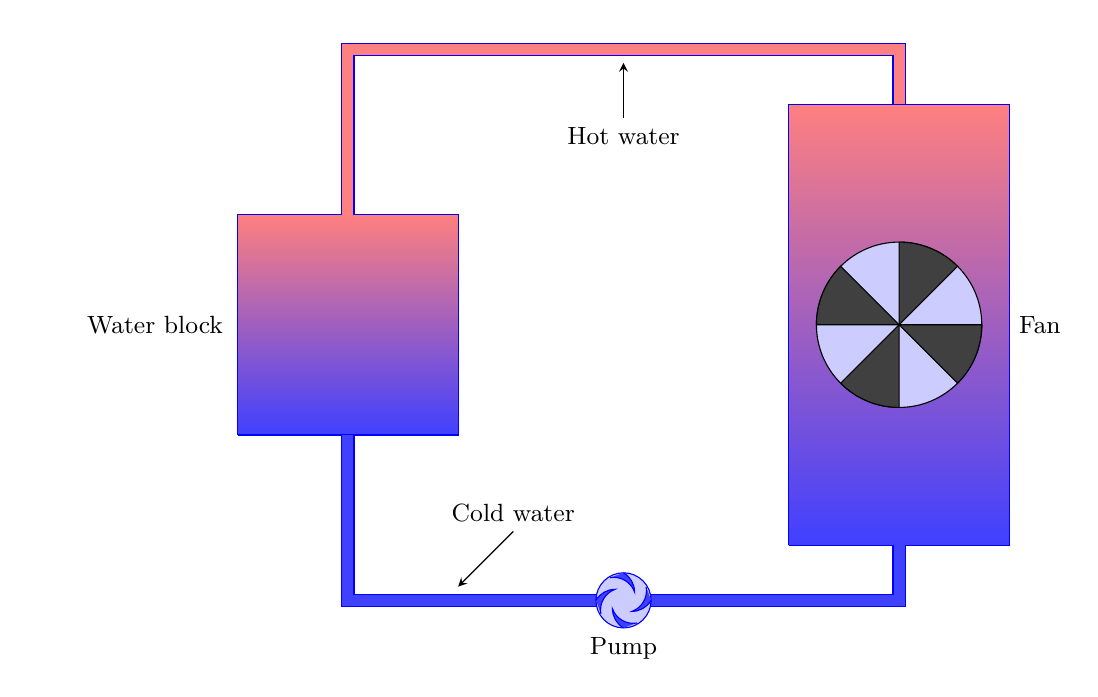
\begin{tikzpicture}[
        scale=0.7,
        annotline/.style = {stealth-},
        arrows1loop/.style={->,red},
        arrows2loop/.style={->,white},
        arrows3loop/.style={->,draw=Gray}]
        \begin{scope}
            % water block
            \filldraw[draw=blue,bottom color=blue!75,top color=red!50] (0, 0) --
            (4, 0) -- (4, 4) -- (0, 4) -- (0, 0);
            % radiator
            \filldraw[draw=blue,bottom color=blue!75,top
            color=red!50,xshift=10cm,yshift=-2cm] (0, 0) -- (0, 8) -- (4, 8) -- (4, 0)
            -- (0, 0);
            % circuit hot
            \draw[draw=blue,double=red!50,double distance=4pt] (2, 4) -- ++(0, 3) --
            ++(10, 0) -- ++(0, -1);
            % circuit cold
            \draw[draw=blue,double=blue!75,double distance=4pt] (2, 0) -- ++(0, -3) --
            ++(10, 0) -- ++(0, 1);
            % arrows
            \draw[arrows2loop] (3.5,-1.3) -- (3,-1.3);
            \draw[arrows2loop] (1.75,-0.9) -- (1.75,-0.4);
            \draw[arrows2loop] (4.5,6.38) -- (5,6.38);
            \draw[arrows2loop] (7,7.38) -- (7.5,7.38);
            \draw[arrows2loop] (8.75,6.4) -- (8.75,5.9);
            \draw[arrows2loop] (8.75,-0.4) -- (8.75,-0.9);
            
            \draw[annotline] (7, 6.75) -- ++(0, -1)
                node[text width=2cm,text centered, font=\small,below] {Hot water};
            \draw[annotline] (4, -2.75) -- ++(1, 1)
                node[text width=2cm,text centered, font=\small,above] {Cold water};
                
            % pump
            \begin{scope}[xshift=7cm,yshift=-3cm]
                \filldraw[fill=Blue!20,draw=Blue] (0,0) circle (0.5cm);
                \node[below,font=\small] at (0,-0.5) {Pump};
                \filldraw[fill=Blue!75,draw=Blue,yshift=-0.5cm]
                    (0,0) arc (240:180:0.4cm)  arc (200:280:0.4cm) ;
                \filldraw[fill=Blue!75,draw=Blue,yshift=+0.5cm,rotate=180]
                    (0,0) arc (240:180:0.4cm)  arc (200:280:0.4cm) ;
                \filldraw[fill=Blue!75,draw=Blue,xshift=+0.5cm,rotate=90]
                    (0,0) arc (240:180:0.4cm)  arc (200:280:0.4cm) ;
                \filldraw[fill=Blue!75,draw=Blue,xshift=-0.5cm,rotate=-90]
                    (0,0) arc (240:180:0.4cm)  arc (200:280:0.4cm) ;
            \end{scope}
            
            % fan
            \begin{scope}[xshift=12cm,yshift=2cm]
                \filldraw[fill=blue!20,draw=black] (0,0) circle (1.5cm);
                \node[right,font=\small] at (2,0) {Fan};
                \filldraw[fill=black!75,draw=black]
                    (0, 0) -- ++(0, 1.5) arc (90:45:1.5cm) -- (0, 0);
                \filldraw[fill=black!75,draw=black]
                    (0, 0) -- ++(1.5, 0) arc (0:-45:1.5cm) -- (0, 0);
                \filldraw[fill=black!75,draw=black]
                    (0, 0) -- ++(0, -1.5) arc (-90:-135:1.5cm) -- (0, 0);
                \filldraw[fill=black!75,draw=black]
                    (0, 0) -- ++(-1.5, 0) arc (180:135:1.5cm) -- (0, 0);
            \end{scope}
            
            \node[text width=3cm,text centered,font=\small] at (-1.5, 2) {Water
            block};
        \end{scope}
    \end{tikzpicture}
    \caption{Schemat technologiczny procesu}
    \label{fig:tech}
\end{figure}